\section{Theory}
\label{sec:Theory}



\subsection{Polyurethane}

Polyurethanes (PUR) are biocompatible and biostable polymers, with urethane as the characteristic group. Due to most PUR being classically synthesised using polycondensation of diisocyanates with alcohols and amines, two side groups per monomer are introduced. This leaves the option for functionalization, depending on the requirement of the application.

\begin{figure}[H]
\centerline{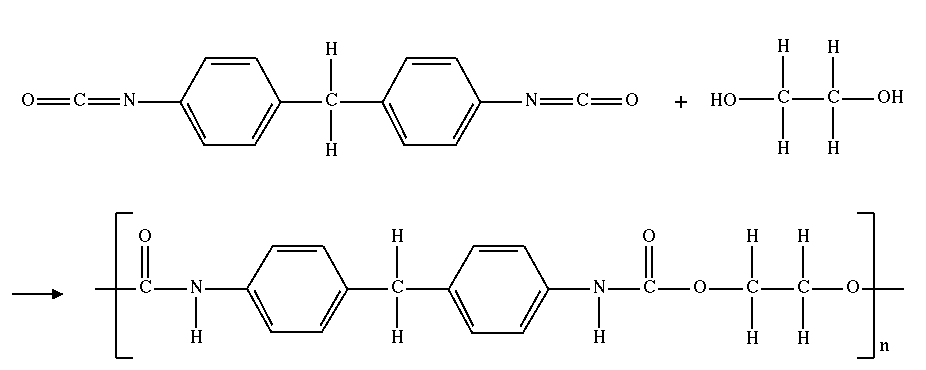
\includegraphics[scale=0.4]{./pic/Polyurethane.png}}
    \caption{Schematic of PUR-Synthesis}
    \label{fig:PURSynth}
\end{figure}

On one hand, they're moldable and have favourable tensile and fatigue properties, all of which makes them a suitable choice of material for the development of most complex biomedical devices. \cite{Pinchuk}
Until now, PUR has been extensively studied in the context of small vascular shunts and cardiac assist devices, where the thromboresistant property of the PUR fit formidable. Under most physiologic conditions, PUR are degradation resistant and can handle stresses very well \cite{Ulery}.

However, PUR, is not electrically conductive. This makes it impossible to introduce electrical functionalities without further processing of PUR, like coating or introducing components with charged side-groups.\cite{Guruthan, Zhu} 


\subsection{Gold Salt}
Our conductive component needs to fulfil multiple requirements. It needs to be biocompatible in all size ranges down to nanoparticle size. This is especially important when considering research on nanoparticles and the associated toxicity, caused through pathophysiological mechanisms.\cite{Buzea, Shukla} Also, we need to be able to incorporate it into our previously non-conductive fiber. In this work, we achieve this through soaking the fiber in a solution where our finally conducting element is dissolved in. Afterwards we want to transform the soluble into a insoluble form and hence fix it inside the fiber through means of a chemical reaction. For the following reasons, Gold is the sensible choice:\\
The biocompatibility is robustly described in literature\cite{Connor, Shukla}, an excellent resistivity ($\rho$ = $2.8*10^{-8}$ $\Omega m$\cite{Principles}) is given and its nanoparticle size and shape is perfectly tunable\cite{Kimling}. Furthermore, there are protocols described, where the intended reduction is achieved by only using biocompatible reducing agents.\cite{Turkevich}\\
Increasing in chemical efficiency is typically achieved by minimising the amount of substance that is wasted in non-targeted interactions. Gold in bulk is highly inert and therefore difficult to incorporate in a directed chemical approach as previously described, whereas the ionic form is a well studied agent in Redox-reactions (i.e.the method that was chosen in this work). The increase in efficiency can be achieved using a spatially selective approach, where gold salt located only in and on the fiber is reduced to become solid gold.\\
Following the same reasoning as in work done by Ngyuen's Group\cite{Nguyen} and others\cite{El-Say, Satis}, Gold(III) chloride trihydrate (i.e. \ce{HAuCl4}) was our decision. 


\subsection{Reducing Agent}
\label{subsec:RedAgent}

Redox-reactions are electrochemical reactions where electrons are exchanged between 
the participating substances. Typically the reaction is described by using two so-called 
half-reactions - the oxidation and the reduction. During reduction, electrons are gained, whereas in oxidation electrons are lost. While the reducing agent reduces the oxidation agent in the process, it gets oxidized. Similar to a kitchen sponge that makes something clean by getting dirty. Additionally, every reduction can also happen in the opposite direction. Experimentally one can derive the likelihood of a reduction happening and assign it a voltage, the so-called standard-reduction-potential or \textsc{SRP}. \\ \vfill \newpage
The \text{SRP} is mostly expressed with respect to the gauge reaction, which is the following: 
 \begin{center}
	\schemestart 
	\ce{[2H]+} + $\mathrm{e^-}$  \arrow{->} \ce{H2}, E\textsuperscript{0}\textsubscript{Hydrogen} = 0.00 V 
	\schemestop\par 
\end{center}

The more negative the SRP of a half-cell, the more likely it is for the half-cell to act as a reduction agent and vice versa.
\\[0.2cm]

 \begin{center}
    \schemestart 
    \ce{[AuCl4]-} + 3$\mathrm{e^-}$  \arrow{->} \ce{Au{(s)}} + 4\ce{Cl-}, E\textsuperscript{0}\textsubscript{Gold} = +0.93 V 
    \schemestop\par 
 \end{center}
 \begin{center}
     \schemestart 
    3Red \arrow{->} 3$\mathrm{Red^+}$ + 3$\mathrm{e^-}$, E\textsuperscript{0}\textsubscript{Red} $\mathrm{<}$ +0.93 V
    \schemestop\par
 \end{center}


The desired reaction to happen, is the reduction of the gold-chloride to get gold in its solid form (denoted by \ce{Au{(s)}}). Gold in bulk is electrically conductive and highly bioinert.
When choosing potential candidates, we defined several qualities, which the desired reducing agent should have.

First, it should reduce gold efficiently and exclusively. On one hand, this confines the list of potentially chosen agents to those who comply with E\textsuperscript{0}\textsubscript{Red} $\mathrm{<}$ +0.93 V, according to Redox-Theory. On the other hand we want to minimise interactions between the reducing agent and PUR, due to possibly modified mechanical, chemical or biocompatible properties. From an efficiency standpoint, we also want to minimise interactions with the solvent.

Second, we want it to be biocompatible. Since the goal of this work lies in applying knowledge in biomedical applications, the importance of biocompatibility is given. If the reducing agents itself fulfils this requirement, then there is no need for introducing a washing-step, which carries the inherent possibility of additional insecurities with its degree of freedom and therefore modes of failure.


Third, the reducing agent should be easily accessible and not too expensive, to facilitate access to technology and faster iterations when further developing to suit the application.

\subsection{Nucleation and Percolation}
\label{subsec:Perc}

When non-polar singular atoms of metallic species are produced in polar liquid, they want to continually aggregate to atoms of the same species, since it's energetically favourable when compared to their existence in the singular atomic state. This leads to the formation of so called embryos.\cite{LaMer} But embryos still mark a non-solid-state phase, since they are subject to a continuous dissociation-aggregation process. If the system allows for an advancement through enough available free energy, eventually the embryos will grow to become nuclei. By further association of metal atoms, the nuclei grow to become primary particles, which as a rule, are still unstable. The diffusion onto them may continue until they form metal particles. Depending on how many primary particles are involved in the production of metal particles, said particles increase up to several micrometers in size. In order to get nanosized particles, a stabilizing agent is needed.\cite{Goia}	
Reducing agents which also act as stabilizing agents therefore will eventually lead to smaller nanoparticles. 

To elucidate how this process is important to us, we have to introduce percolation. Percolation  whose behaviour is governed by laws of Percolation Theory, describes applied to our case the successful transmission of current through a random path, where  each edge (air, PUR) between two nodes (gold nanoparticles) carries a probability of conducting the current. We say that something percolates if the transmission is successful from one end to the other of our sample space. The very important point here is that the exact way through which the current is conducted remains unknown, but the probability. Intuitively, it becomes clear, that in the case of fewer but larger nanoparticles there are fewer but larger overlap with other nanoparticles. This might lead to smaller baseline resistance. However, as soon as we apply strain, those bigger nanoparticles become an uncertainty since the overall percolation depends much more on individual conduction events, leading to a broader probability-distribution of percolation. However, by reasoning of the law of large numbers, in the case of many small nanoparticles the percolation distribution is much narrower, since it depends less on individual contact than more on the overall averaged probability.

Taken those insights from nucleation and percolation together, should lead to one main insight: Namely, that reducing agents, which also act as stabilizers, should lead to less stochastic conductivity, when compared to non-stabilizing reducing agents.

\subsection{Percolation mediated Strain Sensing}

As we have read in the last chapter, percolation leads to conduction. Although, as soon as we apply strain, the distribution of overlap gets more sparse which translates into an increase in resistance increases. The mathematical framework is given by Percolation Theory, which can be read up in an excellent book written by Shante et al.\cite{Shante} The main point of interest is the ratio of the volume of the conductive filler to the volume of the non-conducting polymer composite. For this reason, it is important to include the material dependant poisson's ratio $v$ in your calculations among other things. The most intuitive explanation for the poisson's ratio is given by the following example: When applying transaxial strain, in most cases, a compression in transversal direction can be observed. The ration between those two forces is described by the material dependent Poisson's ratio, which in most cases ranges between 0 and 1. \cite{Gercek}. 